% ----------------------------------------------------------
\chapter{Revisão Bibliográfica}
% ----------------------------------------------------------

Para atingir o objetivo de projetar o \textit{hardware} de uma PCB (\textit{Printed Circuit Board}) de um computador de bordo robusto, foi preciso buscar na literatura acadêmica o estado da arte que tange o projeto de OBDHs (\textit{On-Board Data Handling}) para satélites de pequeno porte, especialmente para CubeSats (satélites de baixo custo, dimensões padronizadas e que utilizam componentes comerciais) (CUBESATS ..., 2022).
 
Primeiro, foi necessário um estudo sobre a radiação em LEO - \textit{Low Earth Orbit} (órbitas com raio menor que 1000 km, segundo ESA, 2024), para que a escolha dos componentes do projeto seja a melhor possível. Com esse estudo, buscaram-se formas de mitigar os efeitos mais conhecidos e verificar como instituições têm lidado com componentes do tipo \textit{commercial-off-the-shelf} (COTS).% Além disso, também foi dada a fundamentação dos conversores de potência, tipos de memória, microprocessadores e interfaces de comunicação.

Depois, foram analisadas as placas de OBDH dos projetos do FloripaSat-1 e FloripaSat-2, desenvolvidas pelo SpaceLab da UFSC. Por fim, outros projetos comerciais foram estudados para obtenção de noções sobre a arquitetura e componentes usados. Um panorama geral foi feito, verificando-se principalmente os componentes principais e mais críticos, ou seja, processadores, memórias voláteis e não-voláteis e outros periféricos.

\section{Radiação em LEO e Componentes COTS}

Estando em solo terrestre, os eletrônicos atuais estão bem protegidos contra a maior parte da radiação incidente do universo. No caso dos satélites orbitais, a proteção atmosférica é atenuada pela distância em relação ao solo, mesmo para aqueles que operam em LEO. Nesse caso, a radiação pode ser suficientemente significativa para causar a mudança do comportamento eletromagnético dos materiais, causando efeitos como falhas, aquisição ou execução errada de comandos e distorção da corrente elétrica (MAYANBARI, 2011).  Esses danos são divididos em dois grupos (JUNQUEIRA, 2020): os acumulativos como o TID (\textit{Total Ionizing Dose}), e os SEE (\textit{Single Event Effects}), que indicam o acontecimento de eventos únicos. 

Ainda segundo Junqueira (2020), o TID se caracteriza principalmente pela formação de pares elétron-lacuna, onde o primeiro aumenta a condutividade do material e o segundo contribui para oxidação, mudando as características elétricas do componente com o tempo.  Já os SEE ocorrem quando um íon atravessa um componente crítico, gerando uma linha de ionização que pode ou não ser destrutiva. 

Por esse motivo, quando são escolhidos os componentes críticos para o \textit{hardware} de um \textit{CubeSat}, em sua maioria COTS, deve-se levar em consideração algumas diretrizes cruciais. Segundo Carmo et al. (2021), o componente escolhido precisa atender os requisitos operacionais, concomitante ao gerenciamento de riscos com mitigações e blindagens. 

Com isso, é possível ver três formas confiáveis de escolher cada componente: usando as diretrizes da ESA (\textit{European Space Agency}), as da NASA (\textit{National Aeronautics and Space Administration}) e também através da herança de voo, ou seja, escolhendo componentes que já estiveram em missões semelhantes ou mais críticas. Nos dois primeiros casos, a consulta é através da norma ECSS-Q-ST-60C para a ESA e da lista NPSL (\textit{NASA Part Selection List}) para a NASA.  No caso da herança de voo, outros projetos devem ser analisados e consultados, o que será feito na seção a seguir.

%\section{Conversores de potência}

%Também chamados de conversores DC-DC, são uma peça crucial em um projeto de PCB. Através de uma tensão de entrada, conseguem convertê-la em tensões maiores ou menores, conforme a necessidade do projetista. Existem diferentes tipos de conversores DC-DC, e tratar-se-á apenas dos conversores chaveados \textit{step-up} e \textit{step-down} nessa seção. 

%\subsection{Conversores \textit{step-up}}

%\section{Memória}

%\section{Microprocessadores}

%\section{Interfaces de comunicação}

\section{Projetos Anteriores}

\subsection{FloripaSat-1}
% https://ieeexplore.ieee.org/abstract/document/9085277
O FloripaSat-1 é uma plataforma \textit{open-source} para nanossatélites. Essa plataforma consiste em três módulos: um módulo de fornecimento de potência (EPS), um computador de bordo (OBDH) e um módulo de telemetria e comunicação (TTC) (MARCELINO et al., 2020).

Seu OBDH foi feito para realização da interface e comunicação entre os módulos e \textit{payloads}. Aqui, destacam-se os sensores presentes: uma \textit{Inertial Measurement Unit} (com giroscópio, magnetômetro e acelerômetro), a interface com os sensores dos painéis solares e as medições de tensão e corrente de entrada do próprio módulo.

Além disso, contava com um microprocessador de 16 bits, memórias flash (IS25LP128) e suporte para cartão microSD para armazenamento.

\subsection{FloripaSat-2}
% https://ieeexplore.ieee.org/abstract/document/10078027
O FloripaSat-2 é a segunda geração da plataforma \textit{open-source} desenvolvida pelo SpaceLab, baseando-se no projeto FloripaSat-1 e trazendo melhorias para os três módulos principais (MARCELINO et al., 2024). O diagrama de blocos do CubeSat proposto está disposto na Figura \ref{fig:floripasat2}, onde pode-se verificar as interfaces do OBDH com o restante do módulo.

\begin{figure}[H]
    \centering
    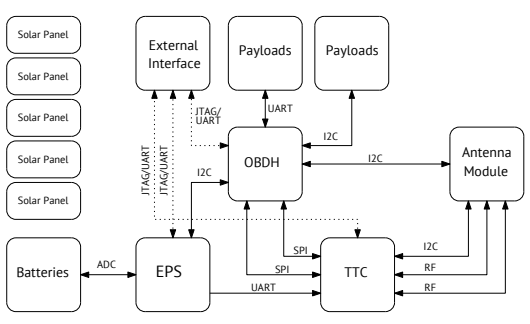
\includegraphics[scale=0.8]{images/floripasat2.png}
    \caption{Diagrama de blocos da plataforma FloripaSat2.}
    \label{fig:floripasat2}
    \fonte{MARCELINO et al., 2024.}
\end{figure}

Especificamente para o OBDH, forami introduzidas uma memória FRAM e uma Flash NOR, ao invés das Flashs e cartão microSD anteriores, o que mostra uma melhoria clara de capacidade e confiabilidade. Outras duas melhorias importantes foram, primeiramente, a adição de um conector para eventualmente conectar uma \textit{daughter board} à placa, e, segundamente, a adição de \textit{buffers} às trilhas de I2C entre os módulos. Isso acrescenta flexibilidade e confiabilidade ao OBDH da segunda geração.

\subsection{Projetos Comerciais}

Abaixo se encontram sintetizados os projetos comerciais estudados, para obtenção de noções sobre a arquitetura e componentes usados. Foram verificados principalmente os processadores, as memórias voláteis e não-voláteis, as interfaces de comunicação e outros periféricos (ADCs, RTC, etc.) utilizados. A Tabela \ref{tab:Tab_Rev} abaixo mostra a pesquisa realizada sobre o Estado da Arte, em conjunto com os dados de George e Wilson (2018), sintetizados na Tabela \ref{tab:Tab_Missoes}.

\begin{table}[htb]
    \centering
	\ABNTEXfontereduzida
	\caption{\label{tab:Tab_Rev}Principais componentes usados pelos fabricantes de OBDHs comerciais.}
	%\begin{tabular}{@{}p{2cm}p{2cm}p{2cm}p{2cm}p{2cm}p{2cm}p{3cm}@{}}
    \begin{tabular}{@{}p{2cm}p{2.6cm}p{2cm}p{2cm}p{2.2cm}p{2.6cm}@{}}
		\toprule
		\textbf{Fabricante} & \textbf{Nome do Produto} & \textbf{Processador} & \textbf{Memórias} & \textbf{Periféricos} & \textbf{Interfaces de comunicação} \\ 
        \midrule
        GomSpace & NanoMind A3200 & AT32UC3C & Flash, SDRAM, FRAM & Giroscópio, Magnetômetro, Transceivers, Sensores de temperatura & CAN, I2C, SPI, JTAG, USART \\%https://gomspace.com/UserFiles/Subsystems/datasheet/gs-ds-nanomind-a3200_1006901-117.pdf
        
        \midrule
        GomSpace & NanoMind HPMK3 & Zynq 7030 & Flash, eMMC, DDR3 & Watchdog, Sensores de temperatura, VCO, Sensores de tensão e corrente & CAN, USART, USB, I2C, JTAG, LVDS, SpaceWire \\ %https://gomspace.com/UserFiles/Subsystems/datasheet/gs-ds-NanoMind_HP_MK3.pdf

        \midrule
        ISIS Space & ISIS On Board Computer & Atmel & Flash, SDRAM, FRAM, Cartões SD & Sensores de temperatura, Sensores de tensão e corrente, RTC, ADC & USART, USB, I2C, JTAG, PWM \\ %https://www.isispace.nl/product/on-board-computer/

        \midrule
        Nano Avionics & SatBus 3C2 & Não informado & Flash, FRAM, Cartões SD & Giroscópio, Magnetômetro, Rádio UHF, ADC & CAN, SPI, I2C, USART, PWM, USB \\ %https://nanoavionics.com/cubesat-components/cubesat-on-board-computer-main-bus-unit-satbus-3c2/

        \midrule
        AAC Clyde Space & Kryten-M3 & Smart Fusion 2 SoC & MRAM, eNVM & RTC, Sensores de tensão e corrente & CAN, SPI, I2C, USART, RS422, LVDS \\ %https://www.aac-clyde.space/what-we-do/space-products-components/command-data-handling/kryten-m3       


		
        \\ \bottomrule
	\end{tabular}
	\fonte{Elaboração própria.}
\end{table}

\begin{table}[H]
	\ABNTEXfontereduzida
	\caption{\label{tab:Tab_Missoes}Síntese da tabela apresentada por George e Wilson (2018).}
	%\begin{tabular}{@{}p{2cm}p{2cm}p{2cm}p{2cm}p{2cm}p{2cm}p{3cm}@{}}
    \centering
    \begin{tabular}{@{} >{\centering}p{3.5cm} >{\centering}p{3.5cm} >{\centering}p{3.5cm} @{}}
    
		\toprule
		\textbf{Fabricante} & \textbf{Processadores} & \textbf{Missões por Fabricante} \tabularnewline 
        \midrule
        Xilinx & Zynq 7020, Zynq 7030, Zynq 7045, Ultrascale+, etc. & 24 \tabularnewline
        
        \midrule
        Atmel + Microchip & ATmega329P, AT91SAM9G20, PIC24F, etc. & 22 \tabularnewline 

        \midrule
        Texas Instruments & MSP430, OMAP3530, Sitara AM3703, etc. & 15 \tabularnewline 

        \midrule
        Cobham Gaisler & GR712RC, UT699, LEON3FT & 8 \tabularnewline
        
        \bottomrule
	\end{tabular}
	\fonte{Elaboração própria com base em George e Wilson, 2018, página 463.}
\end{table}

Comparando ambas tabelas, é possível verificar que a maioria dos processadores apresentados são de duas fabricantes: Xilinx (especialmente \textit{chips} da família Zynq 7000) e Microchip (incluindo Atmel). Além disso, a maior parte dos projetos comerciais vistos apresentam memórias FRAM, que possuem um número máximo de ciclos de leitura e escrita muito elevada, além de memórias Flash. Outro destaque foi a presença de sensores de tensão e corrente, bem como magnetômetros e giroscópios.

Além disso, projetos como o OBDH Nanomind Z7000 (Gomspace Nanomind Z7000 Datasheet, 2019) demonstraram sua efetividade em diversas missões, como FSSCAT (CAMPS et al., 2018), ORCA (BARLES et al., 2022) e CubeMAP (WEIDMANN et al., 2020), o que mostra a confiabilidade e herança de voo de \textit{hardwares} contendo o SoCs da família Zynq 7000. Na Figura \ref{fig:nanomind}, podemos verificar o diagrama de blocos do anteriormente citado Nanomind Z7000.

\begin{figure}[H]
    \centering
    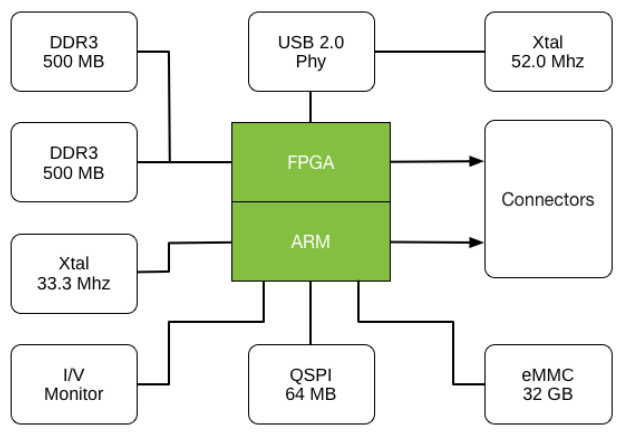
\includegraphics[scale=0.8]{images/nanomind z7000.png}
    \caption{Diagrama de blocos do OBDH Nanomind Z7000.}
    \label{fig:nanomind}
    \fonte{Gomspace Nanomind Z7000 Datasheet, 2019.}
\end{figure}

\subsection{Projetos Acadêmicos}

Outro ponto são os OBDHs propostos em publicações acadêmicas. Serão estudados quatro casos de design de OBDH, ainda no contexto de nanossatélites. 

No primeiro caso, o OBDH foi feito para ser compacto e reconfigurável, como o projeto proposto nesse trabalho. O sistema foi pensado para conter um processador, SDRAMs, uma Flash NOR, uma Flash NAND, uma FPGA e algumas interfaces externas (ZHOU et al., 2018). O diagrama de blocos do OBDH proposto pelos autores está disposto na Figura \ref{fig:zhou}.

\begin{figure}[H]
    \centering
    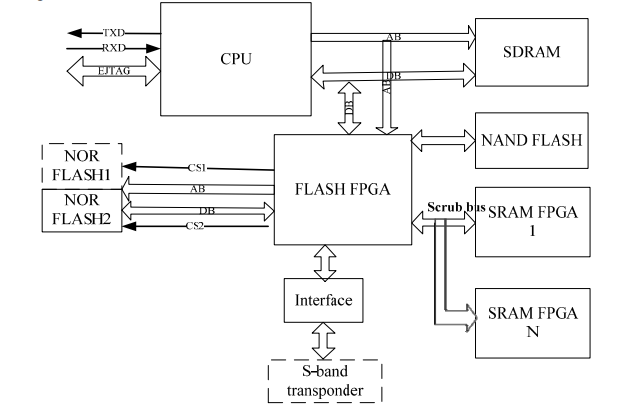
\includegraphics[scale=0.8]{images/zhou.png}
    \caption{Diagrama de blocos do OBDH proposto por ZHOU et al., 2018.}
    \label{fig:zhou}
    \fonte{ZHOU et al., 2018.}
\end{figure}

Na segunda publicação estudada, o OBDH é parte de um sistema que implementa um sistema operacional em tempo real (RTOS), outro objetivo desse trabalho. Nesse caso, o OBDH é capaz de verificar telecomandos, sincronizar sistemas, reportar eventos e monitorar parâmetros (PUTRA, 2021). Seu diagrama de blocos do \textit{hardware} está disposto na Figura \ref{fig:putra}.

\begin{figure}[H]
    \centering
    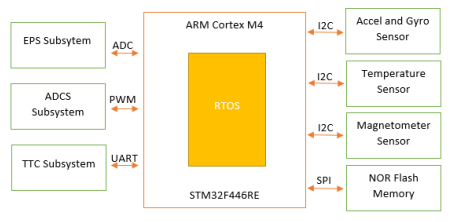
\includegraphics[scale=0.8]{images/putra.png}
    \caption{Diagrama de blocos do OBDH proposto por PUTRA, 2021.}
    \label{fig:putra}
    \fonte{PUTRA, 2021.}
\end{figure}

No terceiro caso, a missão incluía a pesquisa e observação em órbita média (MEO), ou seja, em condições mais críticas do que o propósito do OBDH projetado nesse trabalho. Mesmo assim, as noções da arquitetura proposta são muito parecidas com o estado da arte comercial para LEO, usando inclusive um SoC da família Zynq 7000 (LOFFLER, 2021). O diagrama de blocos do OBDH proposto nesse trabalho está disposto na Figura \ref{fig:loffler}.

\begin{figure}[H]
    \centering
    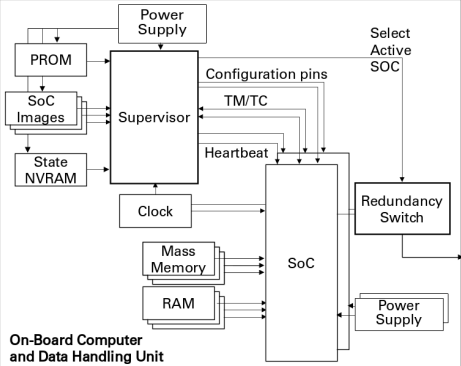
\includegraphics[scale=0.8]{images/loffler.png}
    \caption{Diagrama de blocos do OBDH proposto por LOFFLER et al., 2021.}
    \label{fig:loffler}
    \fonte{LOFFLER et al., 2021.}
\end{figure}

Nos três casos existem semelhanças na arquitetura, incluindo memórias usadas e interfaces de comunicação. Com isso, juntamente com o estudo dos projetos FloripaSat-1 e FloripaSat-2 e projetos comerciais, é possível começar a projetar o \textit{hardware} do OBDH, utilizando as diretrizes citadas e as heranças de voo, tomando como base os projetos citados, escolhendo os componentes e respeitando os requisitos impostos.







% Citação: 
% https://sci-hub.se/10.1109/jproc.2018.2802438
 

